\documentclass{article}

\usepackage{tikz}

\usetikzlibrary{decorations}

\usepackage[EULERGREEK]{sansmath}

\usepackage{etoolbox}

\usepackage[margin=.2in]{geometry}

\usepackage{tabu}

\usepackage{xfrac}

\makeatletter

\def\mute{x}
\def\open{o}
\def\empty{-}
\def\base{I}

% Fix baseline when drawing tikz in side tabu
\tikzset{my pic adjust/.style={%%
  baseline=(my center),
  execute at end picture={\path (current bounding box.north) -- ++ (0,4pt);
                          \path (current bounding box.south) -- ++ (0,-4pt);
                          \path (current bounding box.center) -- ++ (0,#1) coordinate (my center);
                          }%
  },
my pic adjust/.default=0pt,
}

\newrobustcmd{\akkoord}[3][I] {
  \begin{tikzpicture}[font=\sffamily\sansmath, scale=0.35, every node/.style={transform shape}, baseline=(current bounding box.north), my pic adjust=-2pt, yscale=-1] % Note: yscale -1 and node transform shape turns around the texts. this is solved by adding yscale -1 to node (see below)
  % Draw snares and frets (6 and 4)
  \draw[help lines] (0,0) grid (5,4);
  % Write position
  \draw (-1, 0.5) node {\Huge #1};
  \ifx#1\base {

  } \else {
    \draw[thick] (0,-0.1) -- (5,-0.1);
  } \fi
  % Write name of chord
  \node[yscale=-1] at (2.5,-1.5) {\Huge #3};
  % Draw fingers
  \foreach \x/\y/\z [count=\i] in {#2} {
    \ifx\x\mute {
      \node[yscale=-1] at (\i-1, -0.5) {\Large X};
    } \else {
      \ifx\x\open {
        \node[yscale=-1] at (\i-1, -0.5) {\Large O};
        \ifx\y\empty {
          \relax
        } \else {
          \node[yscale=-1] at (\i-1, 4.5) {\Large \y};
        } \fi
      } \else {
        % Find out if we can draw a bar...
        \ifcsdef{@barLowSnare@\y} {
          \csnumgdef{@barHighSnare@\y}{\i}
          \csnumgdef{@barHighFret@\y}{\x}
        } {
          \csnumgdef{@barLowSnare@\y}{\i}
          \csnumgdef{@barLowFret@\y}{\x}
        }
        \filldraw [fill=white] (\i-1, \x-0.5) circle [radius=0.4];
        \node[yscale=-1] at (\i-1, \x-0.5) {\Large \y};
        \ifx\z\empty {
          \relax
        } \else {
          \node[yscale=-1] at (\i-1, 4.5) {\Large \z};
        } \fi
      } \fi
    } \fi
  }
  \foreach \x/\y/\z [count=\i] in {#2} {
    \ifcsdef{@barHighSnare@\y} {
      \draw[thick] (\csuse{@barLowSnare@\y}-1,\csuse{@barLowFret@\y}-0.9) to[out=-20, in=-160] (\csuse{@barHighSnare@\y}-1,\csuse{@barHighFret@\y}-0.9); % Note: because yscale -1 the angles must be turned 180 (-20 and -160)
    }
    \global\csundef{@barLowSnare@\y}
    \global\csundef{@barLowFret@\y}
    \global\csundef{@barHighSnare@\y}
    \global\csundef{@barHighFret@\y}
  }
  \end{tikzpicture}
}

\makeatother

\begin{document}

\begin{tabu}{ X[1,c,m] | X[5,l,m] | X[8,l,m] }
  \textbf{chord} & \textbf{root 6} & \textbf{root 5} \\ \hline
  \textbf{Maj7 \newline $\triangle$} &
  \akkoord[II]{2/1/1,x,3/3/{$\sharp$7},3/4/3,2/2/5,x}{G\textsubscript{$\triangle$}} &
  \akkoord[II]{x,2/1/1,4/3/5,3/2/{$\sharp$7},4/4/3,x}{C\textsubscript{$\triangle$}} \\ \hline
  \textbf{7} &
  \akkoord[II]{2/1/1,x,2/2/7,3/4/3,2/3/5,x}{G\textsubscript{7}}
  \akkoord{3/2/1,x,3/3/7,1/1/{$\flat$9},3/4/5,x}{G\textsubscript{7$\flat$9}} &
  \akkoord[II]{x,2/1/1,4/3/5,2/1/7,4/4/3,2/1/{(5)}}{C\textsubscript{7}}
  \akkoord{x,3/3/1,2/2/3,3/4/7,1/1/1,x}{C\textsubscript{7}}
  \akkoord{x,3/2/1,2/1/3,3/3/7,3/4/9,3/4/{(5)}}{C\textsubscript{79}}
  \akkoord{x,3/4/1,2/3/3,2/2/6,1/1/1,x}{C\textsubscript{6}}\\ \hline
  \textbf{m7\newline-7} &
  \akkoord[II]{2/2/1,x,2/3/7,2/3/{$\flat$3},2/3/5,x}{G-\textsubscript{7}}
  \akkoord{3/1/1,x,2/2/6,3/3/{$\flat$3},3/4/5,x}{G-\textsubscript{6}} &
  \akkoord[II]{x,2/1/1,4/3/5,2/1/7,3/2/{$\flat$3},2/1/{(5)}}{C-\textsubscript{7}}
  \akkoord{x,3/2/1,1/1/{$\flat$3},3/3/7,4/4/{$\flat$3},x}{C-\textsubscript{7}} \\ \hline
  \textbf{-7$\flat$5 m7$\flat$5 \o \newline halfdim.} &
  \akkoord{3/2/1,x,3/3/7,3/4/{$\flat$3},2/1/{$\flat$5},x}{G\textsubscript{\o}} &
  \akkoord[II]{x,2/1/1,3/3/{$\flat$5},2/2/7,3/4/{$\flat$3},x}{C\textsubscript{\o}} \\ \hline
  \textbf{o dim.} \textit{\tiny all notes root, all dist. 1\sfrac{1}{2}} &
  \akkoord{3/2/1,x,2/1/{$\flat$7},3/3/{$\flat$3},2/1/{$\flat$5},x}{G\textsubscript{o}} &
  \akkoord{x,3/2/1,4/3/{$\flat$5},2/1/{$\flat$7},4/4/{$\flat$3},x}{C\textsubscript{o}} \\ \hline \hline
  chord progression ("trap") &
  \begin{tabu}{X[r] X[l]}
    \multicolumn{2}{c}{scale of G: G A B C D E F$\sharp$} \\
    I & G\textsubscript{$\triangle$} \\
    II & A-\textsubscript{7} \\
    III & B-\textsubscript{7} \\
    IV & C\textsubscript{$\triangle$} \\
    V & D\textsubscript{7} \\
    VI & E-\textsubscript{7} \\
    VII & F$\sharp$\textsubscript{o} \\
  \end{tabu} &
  \begin{tabu}{X[r] X[l]}
    \multicolumn{2}{c}{scale of C: C D E F G A B} \\
    I & C\textsubscript{$\triangle$} \\
    II & D-\textsubscript{7} \\
    III & E-\textsubscript{7} \\
    IV & F\textsubscript{$\triangle$} \\
    V & G\textsubscript{7} \\
    VI & A-\textsubscript{7} \\
    VII & B\textsubscript{o} \\
  \end{tabu} \\ \hline
\end{tabu}


\begin{center}
circle of fifths ("kwintencirkel")

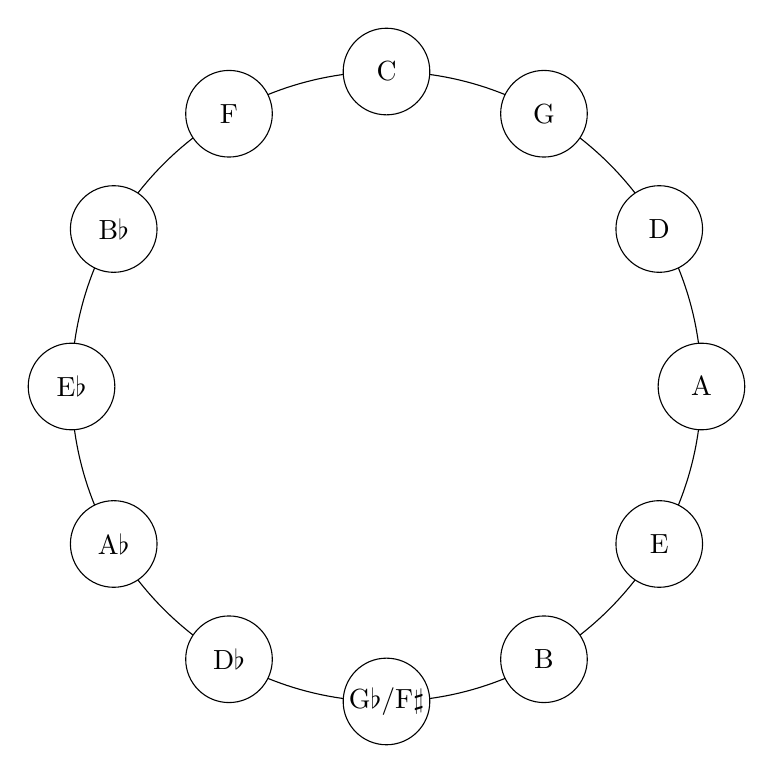
\begin{tikzpicture}
  \draw (0,0) circle [radius=4];
  \filldraw[fill=white] (90:4) circle [radius=.55];
  \filldraw[fill=white] (60:4) circle [radius=.55];
  \filldraw[fill=white] (30:4) circle [radius=.55];
  \filldraw[fill=white] (0:4) circle [radius=.55];
  \filldraw[fill=white] (-30:4) circle [radius=.55];
  \filldraw[fill=white] (-60:4) circle [radius=.55];
  \filldraw[fill=white] (-90:4) circle [radius=.55];
  \filldraw[fill=white] (-120:4) circle [radius=.55];
  \filldraw[fill=white] (-150:4) circle [radius=.55];
  \filldraw[fill=white] (180:4) circle [radius=.55];
  \filldraw[fill=white] (150:4) circle [radius=.55];
  \filldraw[fill=white] (120:4) circle [radius=.55];

  \draw (90:4) node {C};
  \draw (60:4) node {G};
  \draw (30:4) node {D};
  \draw (0:4) node {A};
  \draw (-30:4) node {E};
  \draw (-60:4) node {B};
  \draw (-90:4) node {G$\flat$/F$\sharp$};
  \draw (120:4) node {F};
  \draw (150:4) node {B$\flat$};
  \draw (180:4) node {E$\flat$};
  \draw (-150:4) node {A$\flat$};
  \draw (-120:4) node {D$\flat$};
\end{tikzpicture}
\end{center}
\end{document}
